% Layout elements
\newcommand{\paragraphtitle}[1]{\textsc{#1}\ } % Paragraph title

% Physical constants
\renewcommand{\c}{\mathrm c} % Speed of light
\newcommand{\h}{\mathrm h} % Plank constant
\newcommand{\G}{\mathrm G} % Gravitational constant
\newcommand{\RH}{\mathrm {R_H}} % Hubble radius
\newcommand{\e}{\mathrm e} % Elementary electric charge
\newcommand{\vpty}{\mathrm \varepsilon_0} % Permittivity of the bare vacuum

% Mathematical notations
\let\minusplus\mp % Minus/plus
\newcommand{\eqdef}{:=} % Equals by definition
\newcommand{\IN}{\mathbb{N}} % Integers
\newcommand{\IZ}{\mathbb{Z}} % Relative integers
\newcommand{\IR}{\mathbb{R}} % Real numbers
\newcommand{\IC}{\mathbb{C}} % Complex numbers
\newcommand{\IntRange}[2]{\Lbrack{#1},{#2}\Rbrack} % Integer range
\renewcommand{\exp}[1]{\mathrm{exp} \left( {#1} \right)} % Exponential function
\renewcommand{\ln}[1]{\mathrm{ln} \left( {#1} \right)} % Logarithm function
\renewcommand{\sin}[1]{\mathrm{sin} \left( {#1} \right)} % Sine function
\renewcommand{\cos}[1]{\mathrm{cos} \left( {#1} \right)} % Cosine function
\newcommand{\sinc}[1]{\mathrm{sinc} \left( {#1} \right)} % Cardinal sine function
\newcommand{\esinc}[1]{\mathrm{esinc} \left( {#1} \right)} % Exponential cardinal sine function
\renewcommand{\tan}[1]{\mathrm{tan} \left( {#1} \right)} % Tangent function
\renewcommand{\arctan}[1]{\mathrm{arctan} \left( {#1} \right)} % Inverse tangent function
\renewcommand{\i}{\mathrm{i}} % Imaginary unit
\newcommand{\cc}[1]{\overline{#1}} % Complex conjugate
\newcommand{\CC}{\mathrm{c.c.}} % Complex conjugate of preceding
\newcommand{\FT}[1]{\widetilde{#1}} % Fourier transform
\newcommand{\PV}{\mathrm{P.V.}} % Cauchy principal value
\newcommand{\dx}{\mathrm dx} % Infinitesimal variation
\newcommand{\dX}{\mathrm dX} % Infinitesimal variation
\newcommand{\dt}{\mathrm dt} % Infinitesimal duration
\newcommand{\dE}{\mathrm dE} % Infinitesimal energy
\newcommand{\dnp}{\mathrm dp} % Infinitesimal momentum
\newcommand{\dtp}{\mathrm d^3\p} % Infinitesimal 3-momentum
\newcommand{\dtq}{\mathrm d^3\q} % Infinitesimal 3-wave vector
\newcommand{\dO}{\mathrm d\Omega} % Infinitesimal solid angle
\newcommand{\ddt}{\frac{\mathrm d}{\dt}} % Time derivative
\newcommand{\Id}{\mathbb{1}} % Identity
\renewcommand{\matrix}[1]{\begin{pmatrix} #1 \end{pmatrix}} % Matrix
\newcommand{\operp}{\overset{\perp}{\oplus}} % Orthogonal direct sum

% Delta functions
\newcommand{\deltaX}[1]{\delta_{\sv x} \left({#1}\right)}
\newcommand{\deltaE}[2]{\delta^{({#1})}_{t - t_0} \left({#2}\right)}

% Minkowski space-time
\newcommand{\ST}{\mathcal E} % Space-time

\newcommand{\sv}[1]{\boldsymbol{#1}} % 3-vector
\newcommand{\ssp}{\cdot} % Scalar product of 3-vectors
\newcommand{\scp}{\times} % Cross product of 3-vectors
\newcommand{\svc}[2]{{#1}_{#2}} % 3-vector component
\newcommand{\norm}[1]{\|{#1}\|}

\newcommand{\stv}[1]{\boldsymbol{#1}} % 4-vector
\newcommand{\stsp}{\cdot} % Scalar product of 4-vectors
\newcommand{\stvh}[2]{{#1}^{#2}} % Covariant 4-vector component
\newcommand{\stvl}[2]{{#1}_{#2}} % Contravariant 4-vector component

\newcommand{\stt}[1]{\boldsymbol{#1}} % 4-tensor
\newcommand{\stthh}[3]{{#1}^{#2#3}} % Covariant 4-tensor component
\newcommand{\sttll}[3]{{#1}_{#2#3}} % Contravariant 4-tensor component

% Lattice parameters
\newcommand{\N}{\mathrm N} % Lattice size
\renewcommand{\a}{\mathrm a} % Lattice step
\newcommand{\M}[1]{N_{#1}^{max}} % Maximum occupation number for a given particle type

% Lattice notations
\newcommand{\FL}{\IntRange{-\N}{\N}^3} % Lattice
\newcommand{\FLD}{\left( \frac{\IntRange{-\N}{\N}}{1 + 2 \N} \right)^3} % Dual lattice
\newcommand{\ILD}{\left( \frac{\IZ}{1 + 2 \N} \right)^3} % Infinite dual lattice
\newcommand{\eqp}[1]{\underline{#1}} % Equivalent in the dual lattice
\newcommand{\wl}[1]{\stv x_{#1}} % World line
\newcommand{\wlt}[2]{\stv x_{#1}({#2})} % World line with proper time
\newcommand{\wltp}[2]{{\stv x}'_{#1}({#2})} % World line with proper time in alternative reference frame

% Hilbert spaces
\newcommand{\bra}[1]{\left\langle{#1}\right|\ } % Bra
\newcommand{\ket}[1]{\ \left|{#1}\right\rangle} % Ket
\newcommand{\braket}[2]{\left\langle{#1}|{#2}\right\rangle} % Bracket
\newcommand{\op}[1]{\widehat{#1}} % Linear operator
\newcommand{\dop}[1]{\widehat{#1}^{\dagger}} % Dual operator
\newcommand{\wf}[4]{{#1}^{#2}_{#3}\left({#4}\right)} % Wave function

% Particle fields
\renewcommand{\H}{\mathcal H} % Hilbert space
\newcommand{\F}{\mathcal F} % Subspace of final states
\newcommand{\Hn}[1]{\mathcal H_{#1}} % N particles Hilbert space
\newcommand{\Hp}[1]{\mathcal H^{#1}} % One field Hilbert space
\newcommand{\vac}{\Omega} % Vacuum
\newcommand{\bX}[4]{{#1}^{#2}_{{#3}, {#4}}} % Position basis indices
\newcommand{\ketX}[4]{\ket{\bX{#1}{#2}{#3}{#4}}} % Position basis ket
\newcommand{\bFX}[4]{({#1}^{#2}_{{#3}, {#4}})} % Position basis field indices
\newcommand{\ketFX}[4]{\ket{\bFX{#1}{#2}{#3}{#4}}} % Position basis field ket
\newcommand{\bQ}[4]{{#1}^{#2}_{{#3}, {#4}}} % Wave number basis indices
\newcommand{\ketQ}[4]{\ket{\bQ{#1}{#2}{#3}{#4}}} % Wave number ket
\newcommand{\bFQ}[4]{({#1}^{#2}_{{#3}, {#4}})} % Wave number basis field indices

% Particles
\newcommand{\antiparticle}[1]{\overline{#1}} % Antiparticle notation
\newcommand{\neutrino}[1]{\nu_{#1}} % Neutrino notation
\newcommand{\antineutrino}[1]{\atiparticle{\nu}_{#1}} % Anti-neutrino notation

\newcommand{\electron}{e} % Electron
\newcommand{\positron}{\antiparticle \electron} % Positron
\newcommand{\muon}{\mu} % Muon
\newcommand{\antimuon}{\antiparticle \muon} % Anti-muon
\newcommand{\tauon}{\tau} % Tauon
\newcommand{\antitauon}{\antiparticle \tauon} % Anti-tauon

\newcommand{\neutrinoelectron}{\neutrino \electron} % Neutrino electron
\newcommand{\antineutrinoelectron}{\antineutrino \electron} % Anti-neutrino electron
\newcommand{\neutrinomuon}{\neutrino \muon} % Neutrino muon
\newcommand{\antineutrinomuon}{\antineutrino \muon} % Anti-neutrino muon
\newcommand{\neutrinotauon}{\neutrino \tauon} % Neutrino tauon
\newcommand{\antineutrinotauon}{\antineutrino \tauon} % Anti-neutrino tauon
\newcommand{\quarkup}{u} % Quark up
\newcommand{\antiquarkup}{\antiparticle \quarkup} % Anti-quark up
\newcommand{\quarkcharm}{c} % Quark charm
\newcommand{\antiquarkcharm}{\antiparticle \quarkcharm} % Anti-quark charm
\newcommand{\quarktop}{t} % Quark top
\newcommand{\antiquarktop}{\antiparticle \quarktop} % Anti-quark top
\newcommand{\quarkdown}{d} % Quark down
\newcommand{\antiquarkdown}{\antiparticle \quarkdown} % Anti-quark down
\newcommand{\quarkstrange}{s} % Quark strange
\newcommand{\antiquarkstrange}{\antiparticle \quarkstrange} % Anti-quark strange
\newcommand{\quarkbottom}{b} % Quark bottom
\newcommand{\antiquarkbottom}{\antiparticle \quarkbottom} % Anti-quark bottom

\newcommand{\photon}{\gamma} % Photon

% Operators
\newcommand{\Rop}{\op{\sv r}} % Position operator
\newcommand{\Pop}{\op{\sv p}} % Momentum operator
\newcommand{\Hop}{\op{\mathrm H}} % Hamiltonian operator
\newcommand{\HopQED}{\Hop'_{QED}} % QED Hamiltonian operator
\newcommand{\Qop}[1]{\op{Q}_{#1}} % Electric charge operator
\newcommand{\Jop}[1]{\op{\sv J}_{#1}} % Electric current operator
\newcommand{\Vop}[1]{\op{V}_{#1}} % Electric potential operator
\newcommand{\Aop}[1]{\op{\sv A}_{#1}} % Magnetic potential operator
\newcommand{\Uop}[2]{\op{\mathrm U}({#1},{#2})} % Evolution operator
\newcommand{\Um}[4]{\mathrm U_{{#1}{#2}}({#3},{#4})} % Evolution matrix
\newcommand{\Uopn}[3]{\op{\mathrm U}^{({#1})}({#2},{#3})} % Evolution operator to the order n
\newcommand{\Umn}[5]{\mathrm U_{{#1}{#2}}^{({#3})}({#4},{#5})} % Evolution matrix to the order n
\newcommand{\UopK}[2]{\op{\mathrm U}_0({#1},{#2})} % Kinetic evolution operator
\newcommand{\UopI}[2]{\op{\mathrm U}_\I({#1},{#2})} % Evolution operator in the interaction picture
\newcommand{\UopIn}[3]{\op{\mathrm U}_\I^{({#1})}({#2},{#3})} % Evolution operator in the interaction picture to the order n
\newcommand{\Sop}{\op{\mathrm S}} % Scattering operator
\newcommand{\Sm}[2]{\mathrm S_{{#1}{#2}}} % Scattering matrix
\newcommand{\Smn}[3]{\mathrm S_{{#1}{#2}}^{({#3})}} % Scattering matrix to the order n
\newcommand{\Smp}[2]{\mathrm S^{(#1)}_{#2}} % Scattering matrix on a path
\newcommand{\SmE}[2]{\mathrm S^{(#1)}_{t - t_0}\left({#2}\right)} % Scattering matrix on an energy path
\newcommand{\aop}[3]{\op{a^{#1}}_{{#2}, {#3}}} % Annihilation operator
\newcommand{\cop}[3]{\dop{a^{#1}}_{{#2}, {#3}}} % Creation operator
\newcommand{\aAlg}{\mathcal A} % Algebra of the annihilation operators
\newcommand{\cAlg}{\mathcal A^{\dagger}} % Algebra of the creation operators
\newcommand{\Nop}[3]{\op{N^{#1}}_{{#2}, {#3}}} % Particle number operator
\newcommand{\tSAop}[3]{\op{\sv{\psi}^{#1}}_{{#2}, {#3}}} % 3-Spinor annihilation operator
\newcommand{\tSCop}[3]{\dop{\sv{\psi}^{#1}}_{{#2}, {#3}}} % 3-Spinor creation operator
\newcommand{\SAop}[3]{\op{\psi^{#1}}_{{#2}, {#3}}} % 4-Spinor annihilation operator
\newcommand{\SCop}[3]{\op{\overline \psi^{#1}}_{{#2}, {#3}}} % 4-Spinor creation operator
\newcommand{\Faop}[3]{\op{\epsilon^{#1}}_{{#2}, {#3}}} % Fermion antisymmetrization operator
\newcommand{\Pn}[2]{\pi^{#1}_{#2}} % Standard particle numbering function

% Physical notations
\newcommand{\pt}{\phi} % Placeholder particle type
\newcommand{\ptf}{f} % Placeholder fermion particle type
\newcommand{\n}{\sv n} % Placeholder position
\newcommand{\q}{\sv q} % Placeholder wave number
\renewcommand{\sp}{\lambda} % Placeholder spin state
\newcommand{\p}{\sv p} % Placeholder 3-momentum
\newcommand{\E}{E} % Placeholder energy
\newcommand{\Ek}[2]{\E^{#1}_{#2}} % Kinetic energy
\newcommand{\vk}[2]{\sv v^{#1}_{#2}} % Kinetic velocity
\newcommand{\bkn}[2]{\beta^{#1}_{#2}} % Kinetic beta factor
\newcommand{\bk}[2]{\sv \beta^{#1}_{#2}} % Kinetic beta vector
\newcommand{\gk}[2]{\gamma^{#1}_{#2}} % Kinetic gamma factor
\newcommand{\mk}[2]{\mathrm m^{#1}_{#2}} % Kinetic mass
\newcommand{\mkn}[3]{\mathrm m^{#1 ({#3})}_{#2}} % Kinetic mass to the order n
\renewcommand{\mp}[1]{\mathrm m_{#1}} % Rest mass of a bare particle
\newcommand{\mpr}[1]{\mathrm M_{#1}} % Reduced rest mass of a bare particle
\newcommand{\qp}[1]{\mathrm q_{#1}} % Electric charge of a dressed particle
\newcommand{\Qp}[1]{\mathrm Q_{#1}} % Particle electric charge number
\newcommand{\I}{I} % Interaction picture
\newcommand{\TP}[2]{\mathcal P \left( {#1} \to {#2} \right)} % Transition probability
\newcommand{\TPn}[3]{\mathcal P^{({#3})} \left( {#1} \to {#2} \right)} % Transition probability to the order n
\newcommand{\CSn}[3]{\sigma^{({#3})} \left( {#1} \to {#2} \right)} % Cross section to the order n
\newcommand{\V}{V} % Coulomb potential

% Spinors
\newcommand{\sigmat}[1]{\sigma_{#1}} % Pauli matrices
\newcommand{\gammat}[1]{\gamma^{#1}} % Dirac matrices
\newcommand{\gamvec}{\sv \gamma} % Dirac matrices 3-vector
\newcommand{\dirspin}[3]{u^{#1}_{{#2}, {#3}}} % Dirac spinor
\newcommand{\ddirspin}[3]{{u^{#1}}^{\dagger}_{{#2}, {#3}}} % Dual Dirac spinor
\newcommand{\photonspin}[2]{\sv \varepsilon_{{#1},{#2}}} % Photon polarization vector
\newcommand{\cphotonspin}[2]{\sv \varepsilon_{{#1},{#2}}^*} % Conjugate photon polarization vector

% Mental notations
\newcommand{\CMS}{\mathcal M} % Set of all collective mental states
\newcommand{\ims}{\mathfrak{m}} % Placeholder individual mind state
\newcommand{\cms}{\mathfrak{M}} % Placeholder collective mind state
\newcommand{\bM}[2]{{#1}_{#2}} % Mental state indices
\newcommand{\bFM}[2]{({#1}_{#2})} % Mental field indices
\newcommand{\God}{\mathfrak{G}} % God

% Symbols
\newcommand{\ExcitedAtom}{$\vcenter{\hbox{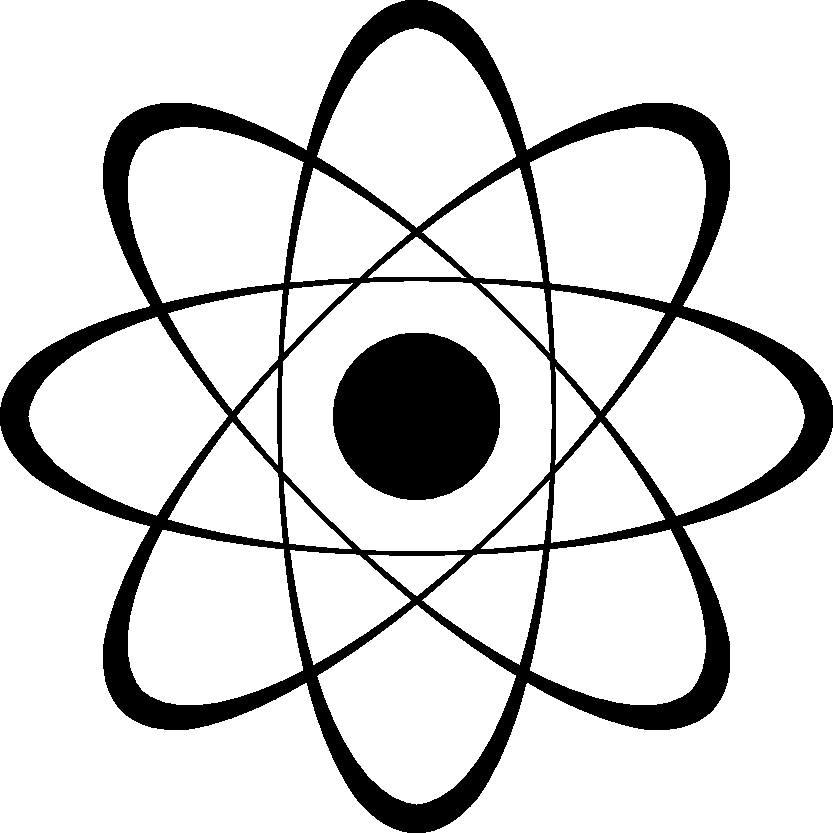
\includegraphics[height=.6cm]{images/pictures/atom.pdf}}}$} % Excited atom
\newcommand{\DetectorOff}{$\vcenter{\hbox{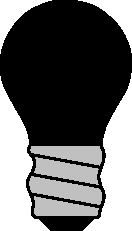
\includegraphics[height=.6cm]{images/pictures/bulb_off.pdf}}}$} % Detector off (waiting)
\newcommand{\DetectorOn}{$\vcenter{\hbox{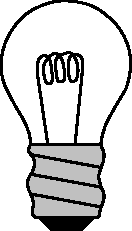
\includegraphics[height=.6cm]{images/pictures/bulb_on.pdf}}}$} % Detector on (activated)
\newcommand{\Atom}{$\vcenter{\hbox{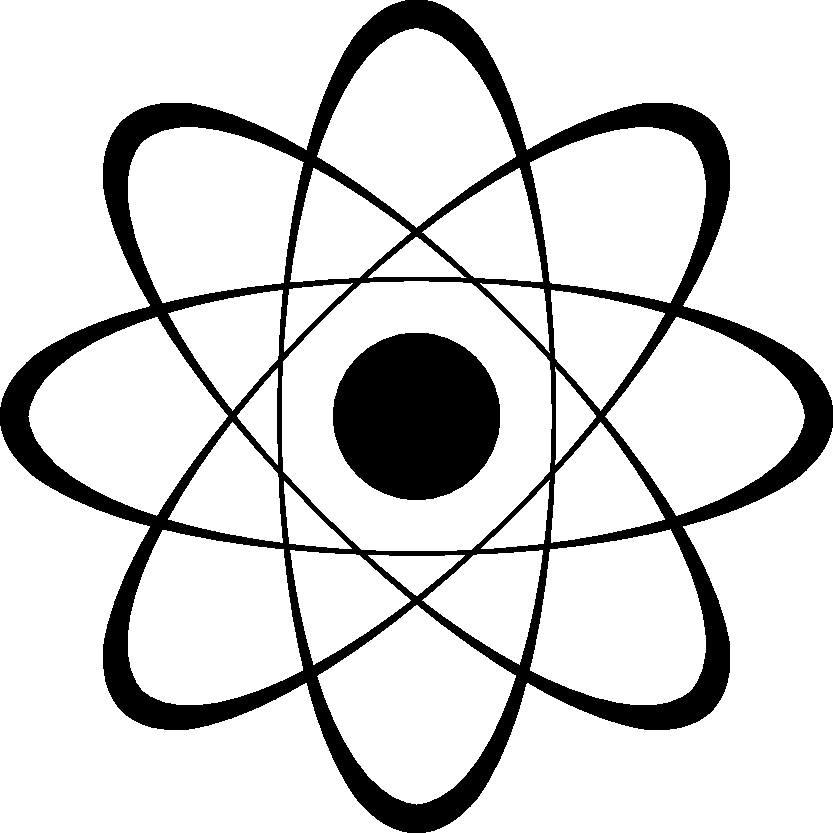
\includegraphics[height=.4cm]{images/pictures/atom.pdf}}}$} % Atom
\newcommand{\Photon}{$\vcenter{\hbox{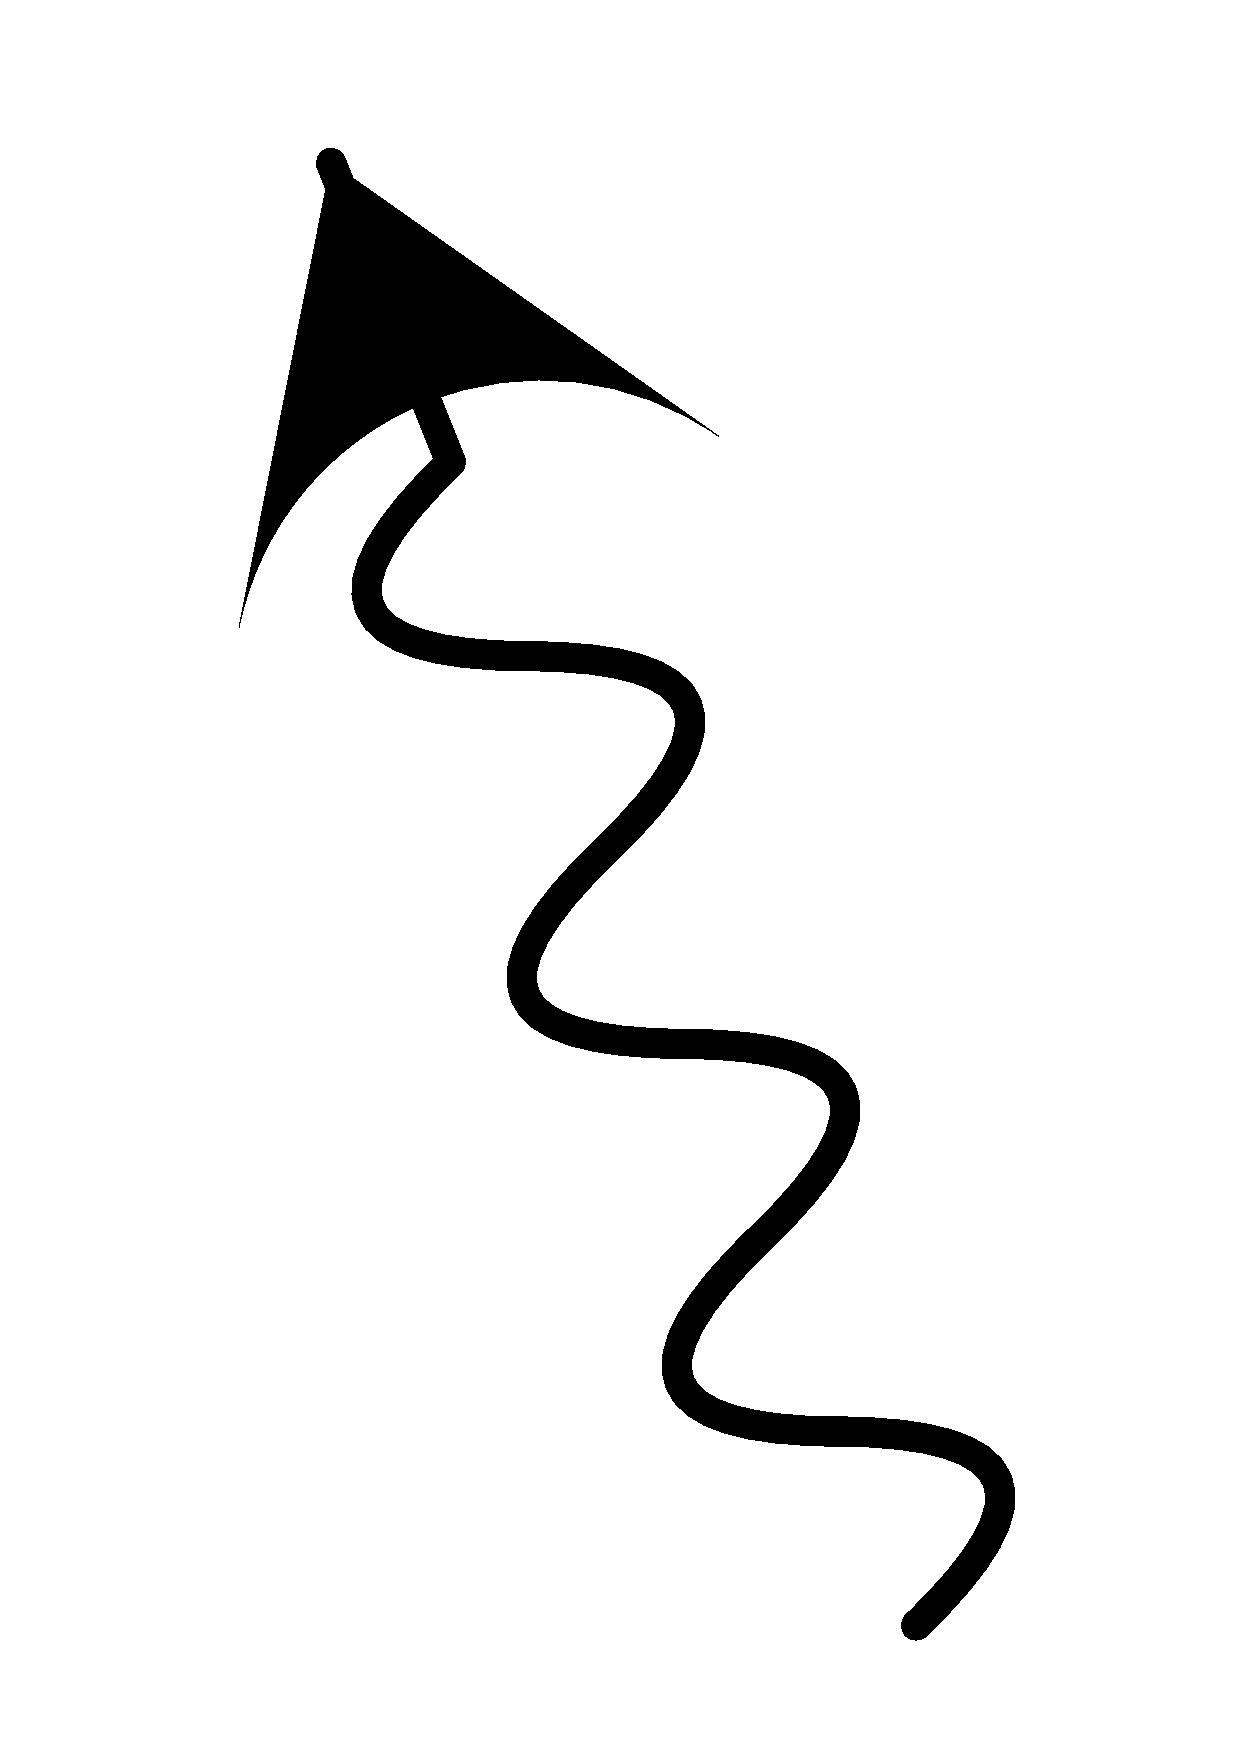
\includegraphics[height=.6cm,angle=-90,origin=c]{images/diagrams/Photon.pdf}}}$} % Photon
\newcommand{\ObserverOff}{$\vcenter{\hbox{\huge\textit?}}$} % Observer off (waiting)
\newcommand{\ObserverOn}{$\vcenter{\hbox{\huge\textit!}}$} % Observer on (having observed the expected result)
\newcommand{\Superposition}{$\vcenter{\hbox{\huge+}}$} % Quantum superposition
